\section{Entwurfsprinzipien}
\label{sec:Kap-7.2}

Im Prozess der Softwareentwicklung geht es auf verschiedenen Ebenen immer wieder darum, Komplexität zu reduzieren. \cite[19]{ous21} gibt eine sehr eingängige und praktische Definition von Komplexität: „Komplexität ist all das, was mit der Struktur eines Soft\-ware\-sys\-tems in Zusammenhang steht und dieses schwer verständlich und schwer anpassbar macht.“

Ein entscheidender Teil der Komplexität in einem Softwaresystem entsteht durch die Beziehungen zwischen den Komponenten. Je nachdem, auf welche Weise und wie stark Komponenten miteinander verbunden sind, wirken sich Änderungen an einer Komponente mehr oder weniger stark auf andere Komponenten aus. Ziel bei der Zerlegung der Systemfunktionalität in Komponenten – sei es als große Komponenten der Architektur, als kleinere Komponenten innerhalb dieser Architektur oder auf der niedrigen Ebene der Klassen – ist es, möglichst wenig Komplexität ins System zu bringen. Wenn alle Komponenten eines Systems völlig unabhängig voneinander wären, indem sich ihre Aufgabenbereiche nicht überschneiden und sie gar nicht miteinander verbunden wären, wäre man auf dem Weg der Komplexitäts\-reduktion schon recht weit – die reine Anzahl der Komponenten und die inhaltliche Komplexität der zu erfüllenden Aufgabe jeder Komponente bliebe natürlich noch. Ein solches System könnte aber fast immer seinen Zweck nicht erfüllen. Die im letzten Abschnitt vorgestellten Architekturmuster und die in diesem Abschnitt beschriebenen Entwurfsprinzipien sind Wege, sich einem komplexitätsreduzierten System, das aber trotzdem seinen Einsatzzweck erfüllt, anzunähern.

\minisec{Komponentenbeziehungen}

Komponenten können in unterschiedlichen Beziehungen zueinander stehen. Abbildung \ref{fig:komponentenbeziehungen} zeigt einige typische Komponentenbeziehungen in Softwaresystemen.

\vspace{\baselineskip} %%% für Druck

\begin{figure}[h!]
	\centering
	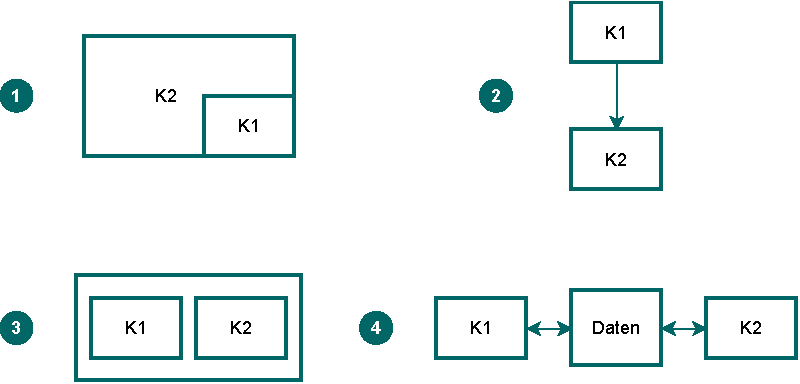
\includegraphics{Bilder/Kapitel-7/komponentenbeziehungen.pdf}
	\caption[Komponentenbeziehungen]{Komponentenbeziehungen, eigene Abbildung in Anlehnung an \cite[105]{som20}}
	\label{fig:komponentenbeziehungen}
\end{figure}

\vspace{\baselineskip} %%% für Druck

\begin{enumerate}
	\item \textbf{ist-Teil-von-Beziehung:} Eine Komponente (K1 in der Abbildung) kann Teil einer anderen Komponente sein (hier K2). So kann zum Beispiel eine bestimmte Operation Teil einer Klasse sein oder eine Klasse zur Zins\-berechnung Teil einer Komponente mit finanzmathematischen Funktionalitäten oder eine Komponente zur Anzeige der Benutzungsoberfläche Teil der Architektur\-komponente Benutzungsschnittstelle.
	\item \textbf{benutzt-Beziehung}: Eine Komponente (K1) verwendet die Funktionalität einer anderen Komponente (K2). Diese Beziehungsart findet man häufig. Auf der Ebene von Klassen und Objekten gehören sämtliche Aufrufe eines Objekts von Operationen anderer Objekte dazu.
	\item \textbf{ist-zusammen-mit-Beziehung:} Zwei Komponenten (K1 und K2) sind in derselben übergeordneten Struktur (das äußere Rechteck) verortet. Auf 
	\linebreak %%% für Druck
	Architekturebene trifft das zum Beispiel auf Komponenten zu, die sich in derselben Schicht einer Schichtenarchitektur befinden.
	\item \textbf{teilt-Daten-mit-Beziehung} Eine Komponente teilt Daten mit einer anderen Komponente. Hier könnte man noch weiter unterscheiden, wie genau dieses Teilen von Daten aussieht, zum Beispiel ob beide Komponenten auf dieselbe Datenbasis zugreifen (so ist es in der Abbildung) oder ob es einen Datenfluss zwischen ihnen gibt etc.
\end{enumerate}

In allen Fällen können die Abhängigkeiten zwischen den Komponenten dazu führen, dass Änderungen bei einer der beiden Komponenten Änderungen an der anderen Komponente nach sich ziehen. Genau das versucht man in der Softwareentwicklung zu vermeiden. Bewährte Entwurfsprinzipien zeigen Strategien auf, wie man trotz dieser Arten von Abhängigkeiten zwischen den Komponenten den Änderungsbedarf an verbundenen Komponenten minimiert.
